\chapter{Length}
 
Recall that a sequence 
\[a=t_0 < t_1 < \cdots < t_k=b.\]
is called a \emph{partition} of the interval $[a,b]$.

\begin{thm}{Definition}\label{def:length}
Let $\gamma\:[a,b]\to \mathcal{X}$ be a curve in a metric space.
The \emph{length}\index{length of curve} of $\gamma$ is defined as
\begin{align*}
\length \gamma
= 
\sup \{|\gamma(t_0)-\gamma(t_1)|&+|\gamma(t_1)-\gamma(t_2)|+\dots
\\
&\dots+|\gamma(t_{k-1})-\gamma(t_k)|\},
\end{align*}
where the supremum is taken over all partitions
\[a=t_0 < t_1 < \cdots < t_k=b.\]

The length of $\gamma$ is a nonnegative real number or infinity;
the curve $\gamma$ is called \emph{rectifiable}\index{rectifiable curve} if its length is finite. 

The length of a closed curve is defined as the length of the corresponding loop.
If a curve is defined on an open or semi-open interval, then its length is defined as the supremum of the lengths of its restrictions to compact intervals.
\end{thm}

If $\gamma$ is a space curve, then its length equals the supremum of the lengths of polygonal lines $p_0\dots p_k$ \emph{inscribed} in the curve (that is, $p_i=\gamma(t_i)$ for a  partition $a=t_0 < t_1 < \cdots < t_k=b$).
If $\gamma$ is closed, then $p_0=p_k$, so the inscribed polygonal line is also closed.


\begin{thm}{Exercise}\label{ex:integral-length}
Let $\gamma\: I \to\RR^3$ ba a curve and $\phi : J \to I$ a homeomorphism. We call the curve $\gamma \circ \phi$ a 
\emph{reparametrization} of $\gamma$. Show that $\length (\gamma \circ \phi ) = \length \gamma$.
\end{thm}





\begin{thm}{Exercise}\label{ex:length-image}
Let $\alpha\:[0,1]\to\RR^3$ be a parametrization of a simple closed arc.
Suppose a path $\beta\:[0,1]\to\RR^3$ has the same image as $\alpha$;
that is, $\beta([0,1])=\alpha([0,1])$.
Show that 
\[\length \beta\ge \length \alpha.\]

\end{thm}


\begin{thm}{Exercise}\label{ex:integral-length}
Assume $\gamma\:[a,b]\to\RR^3$ is a smooth curve.
Show that
\begin{enumerate}[(a)]
\item\label{ex:integral-length>} $\length \gamma\ge \int_a^b|\gamma'(t)|\cdot dt$,
\item\label{ex:integral-length<} $\length \gamma\le \int_a^b|\gamma'(t)|\cdot dt$.
\end{enumerate}
Conclude that 
\[\length \gamma= \int_a^b|\gamma'(t)|\cdot dt.\eqlbl{eq:length}\]
\end{thm}




\section*{Nonrectifiable curves}
A classical example of a nonrectifiable curve is the so-called \emph{Koch snowflake};
it is a fractal curve that can be constructed as follows:

Start with an equilateral triangle, divide each side into three segments of equal length and add an equilateral triangle with base the middle segment.
Repeat this construction recursively with the obtained polygons.
\begin{figure}[h!]
\begin{minipage}{.24\textwidth}
\centering
\vskip5.9mm
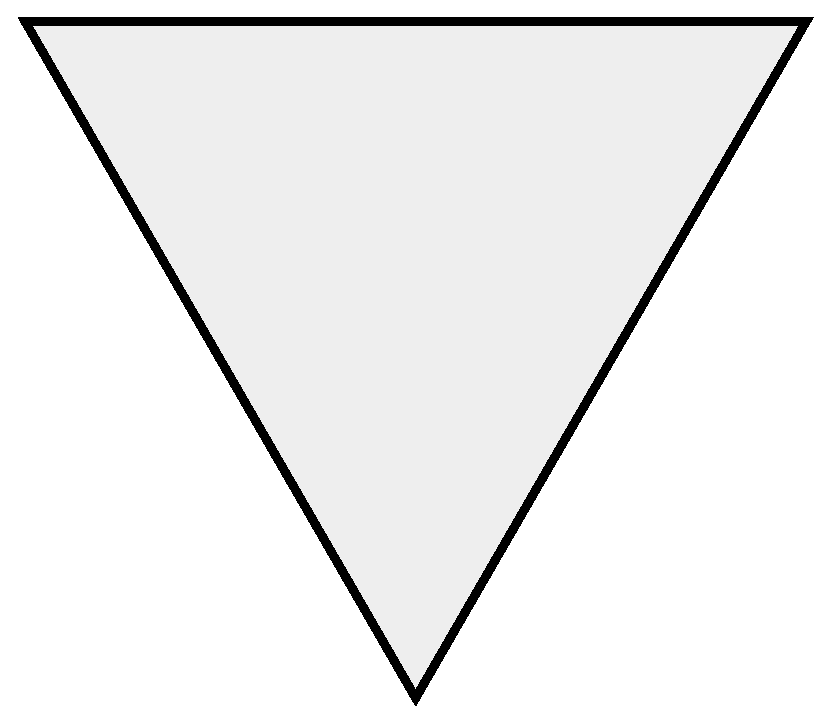
\includegraphics[scale=.15]{pics/Koch_Snowflake-0}
\end{minipage}
\hfill
\begin{minipage}{.24\textwidth}
\centering
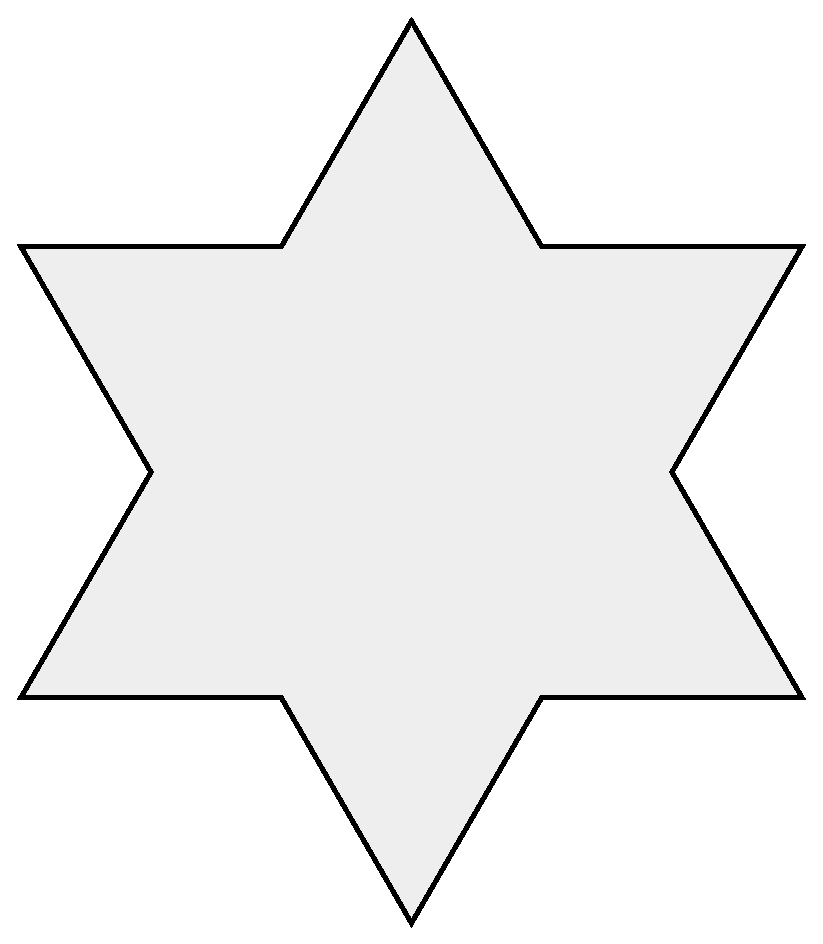
\includegraphics[scale=.15]{pics/Koch_Snowflake-1}
\end{minipage}
\hfill
\begin{minipage}{.24\textwidth}
\centering
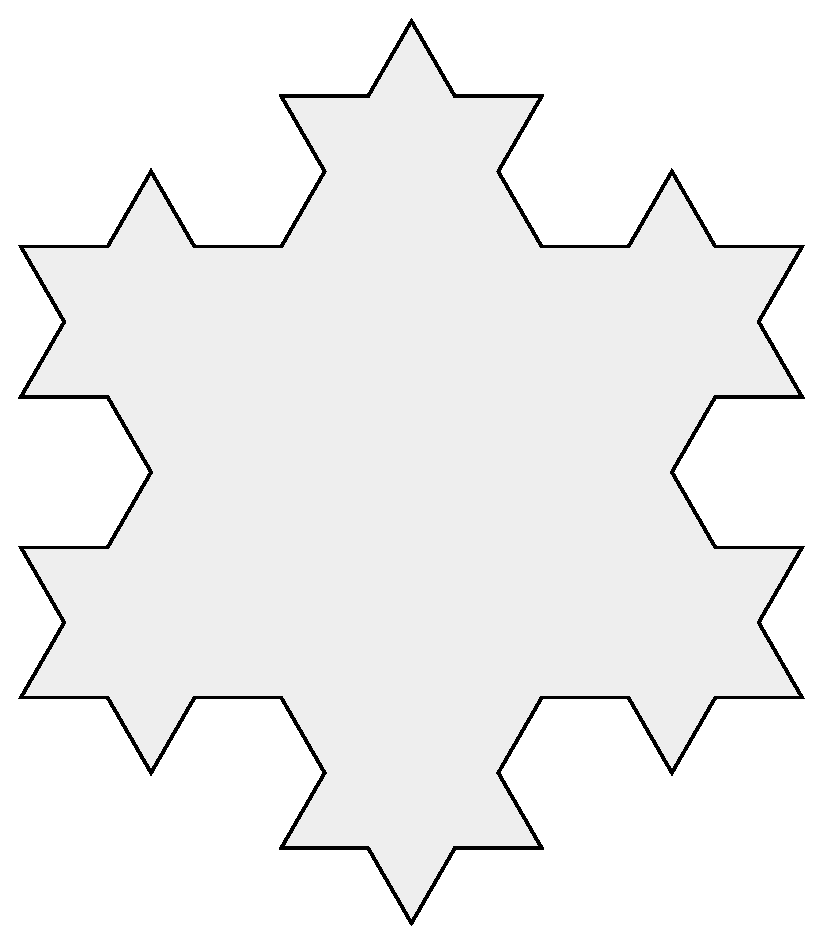
\includegraphics[scale=.15]{pics/Koch_Snowflake-2}
\end{minipage}
\hfill
\begin{minipage}{.24\textwidth}
\centering
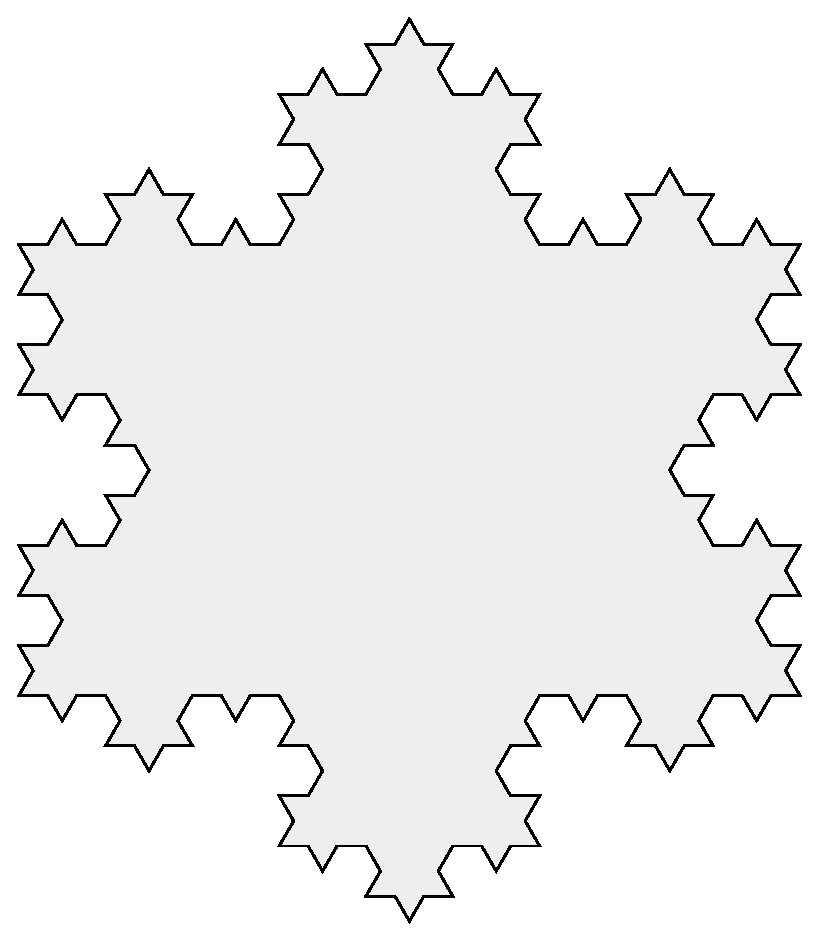
\includegraphics[scale=.15]{pics/Koch_Snowflake-3}
\end{minipage}
\end{figure}
Few first iterations of the construction are shown on the diagram.
The Koch snowflake is the boundary of the union of all the polygons.


\begin{thm}{Exercise}\label{ex:nonrectifiable-curve}
\begin{enumerate}[(a)]
\item Show that the Koch snowflake is a closed simple curve; that is, it can be parameterized by a circle.
\item\label{ex:nonrectifiable-curve:b} Show that the Koch snowflake is not rectifiable. 
\end{enumerate}
\end{thm}
  
  
\section*{Arc length parametrization}

We say that a curve $\gamma$ is an \emph{arc-length parametrization} (also called \emph{natural parametrization})
if for any two values of parameters $t_1<t_2$, the value $t_2-t_1$ is the length of $\gamma|_{[t_1,t_2]}$; that is, the closed arc of $\gamma$ from $t_1$ to $t_2$.

Note that a smooth space curve $\gamma(t)=(x(t),y(t),z(t))$ is an arc-length parametrization if and only if it has unit velocity vector at all times;
that is, 
\[|\gamma'(t)|=\sqrt{x'(t)^2+y'(t)^2+z'(t)^2}=1\]
for all $t$; by that reason smooth curves equipped with an arc-length parametrization are also called \emph{unit-speed curves}.
Note that smooth unit-speed curves are automatically regular.


Any rectifiable curve can be parameterized by arc length.
For a parametrized smooth curve $\gamma : [ t_0 , t_1] \to \mathcal{X}$, the arc-length parameter $s$ can be written as an integral
\[s(t)=\int_{t_0}^t |\gamma'(\tau)|\cdot d\tau.\] %??? s is overloaded
Note that $s(t)$ is a smooth non-decreasing function.
By the fundamental theorem of calculus, $s'(t)=|\gamma'(t)|$.
Therefore if $\gamma$ is regular, then $s'(t)\ne0$ for any parameter value $t$.
By the inverse function theorem (\ref{thm:inverse}) the inverse function $s^{-1}(t)$ is also smooth.
Therefore $\gamma\circ s^{-1}$ remains smooth and regular. It is straightforward to check that $\gamma\circ s^{-1}$ is an arc length parametrization.

Most of the time we use $s$ for an arc-length parameter of a curve.

\begin{thm}{Exercise}\label{ex:arc-length-helix}
Reparametrize the helix 
\[\gamma_{a,b}(t)=(a\cdot\cos t,a\cdot \sin t, b\cdot t)\]
by its arc length.
\end{thm}

We will be interested in the properties of curves that are invariant under a reparametrization.
Therefore we can always assume that any given smooth regular curve comes with an arc-length parametrization.
A nice property of arc-length parametrizations is that they are almost canonical --- these parametrizations differ only by a sign and an additive constant.
By that reason, it is easier to express parametrization-independent quatities using arc-length parametrizations;
this will be usefull in the definition of curvature and torsion.

On the other hand, it is often impossible to find an arc-length parametrization in explicit form, which makes it hard to perform calculations;
usually it is more convenient to use the original parametrization.

\section*{Convex curves}

A simple plane curve is called \emph{convex} if it bounds a convex region.

\begin{thm}{Proposition}\label{prop:convex-curve}
Assume a convex closed curve $\alpha$ lies inside the domain bounded by a simple closed plane curve $\beta$.
Then
\[\length\alpha\le \length\beta.\]
\end{thm}

Note that it is sufficient to show that for any polygon  $P$ inscribed in $\alpha$ there is a polygon $Q$ inscribed in $\beta$ with 
$\perim P\le \perim Q$.

Therefore it is sufficient to prove the following lemma.


\begin{thm}{Lemma}\label{lem:perimeter}
Let $P$ and $Q$ be polygons.
Assume $P$ is convex and $Q\supset P$.
Then 
\[\perim P\le \perim Q.\]

\end{thm}


\begin{wrapfigure}{o}{24 mm}
\vskip-2mm
\centering
\includegraphics{mppics/pic-7}
\vskip2mm
%\caption*{}
\end{wrapfigure}

\parit{Proof.} %??? redo the proof with closest point projection
Note that by the triangle inequality,
the inequality
\[\perim P\le \perim Q\]
holds
if $P$ can be obtained from $Q$ by cutting it along a chord;
that is, a line segment in $Q$ with ends on the boundary of $Q$.


Note that there is an increasing sequence of polygons 
$$P=P_0\subset P_1\subset\dots\subset P_n=Q$$
such that $P_{i-1}$ obtained from $P_{i}$ by cutting along a chord.
Therefore 
\begin{align*}
\perim P=\perim P_0&\le\perim P_1\le\dots
\\
\dots&\le\perim P_n=\perim Q
\end{align*}
and the lemma follows.
\qeds

\begin{thm}{Corollary}
Any convex closed plane curve is rectifiable.  
\end{thm}

\parit{Proof.}
Any closed curve is bounded.
Indeed, the curve can be described as an image of a loop $\alpha\:[0,1]\to\RR^2$, $\alpha(t)=(x(t),y(t))$.
The coordinate functions $x(t)$ and $y(t)$ are continous functions defined on $[0,1]$.
Therefore the absolute values of bothfunctions are bounded by some constant $C$.
Therefore, $\alpha$ lies in the square defined by the inequalities $|x|\le C$ and $|y|\le C$.

By Proposition~\ref{prop:convex-curve}, the length of the curve cannot exceed the perimeter of the square $8\cdot C$, hence the result.
\qeds

Recall that the convex hull of a set $X$ is the smallest convex set that contains $X$; equivalently, the convex hull of $X$ is the intersection of all convex sets containing $X$.

\begin{thm}{Exercise}\label{ex:convex-hull}
Let $\alpha$ be a simple closed plane curve.
Denote by $K$ the convex hull of $\alpha$; let $\beta$ be the boundary curve of $K$.
Show that 
\[\length \alpha\ge \length \beta.\]

Try to show that the statement holds for arbitrary closed plane curves $\alpha$, assuming only that $K$ has nonempty interior.
\end{thm}


\section*{Crofton formulas*}

Consider a smooth plane curve $\gamma\:[a,b]\to\RR^2$.
Given a unit vector $u$, denote by $\gamma_u$ the curve that follows the orthogonal projection of $\gamma$ to the line in the direction $u$;
that is, 
\[\gamma_u(t)=\langle u,\gamma(t)\rangle\cdot u.\]

Note that 
\[|\gamma_u'(t)|=|\langle u,\gamma'(t)\rangle|\] for any $t$.
Note that for any plane vector $w$, the average magnitude of its projections is proportional to its magnitude; that is,
\[|w|=k\cdot \overline{|w_u|},\]
where $\overline{|w_u|}$ denotes the average value of $|w_u|$ for all unit vectors $u$.
(The value $k$ is the average value of $|\cos\phi|$ for $\phi\in [0,2\cdot\pi]$; it can be found by integration, but soon we will show another way to find it.)

If the curve $\gamma$ is smooth, then according to Exercise~\ref{ex:integral-length}
\begin{align*}
\length\gamma
&=\int_a^b|\gamma'(t)|\cdot dt=
\\
&=\int_a^b  k\cdot \overline{|\gamma_u'(t)|}\cdot dt=
\\
&=k\cdot \overline{\length\gamma_u}.
\end{align*}
This formula and its relatives are called \emph{Crofton formulas}.
Since $k$ in universal for any curve, we can take $\gamma$ to be the unit circle to compute $k$: the left hand side is $2\cdot\pi$.
Note that for any unit vector $u$, the curve $\gamma_u$ runs back and forth along an interval of length 2.
Therefore $\length\gamma_u=4$ and hence its average value is also 4.
It follows that the coefficient $k$ has to satisfy the equation $2\cdot \pi =k\cdot 4$; hence 
\[
\length\gamma
=\tfrac\pi2\cdot \overline{\length\gamma_u}.
\]

The Crofton's formula holds for arbitrary rectifiable curves, not necessary smooth; it can be proved using Exercise~\ref{adex:integral-length}.

\begin{thm}{Exercise}\label{ex:convex-croftons}
Show that any closed plane curve $\gamma$ has length at least $\pi\cdot s$, where $s$ is the average length of pojections of $\gamma$ to lines.
Moreover, equality holds if and only if $\gamma$ is convex.

Use this statement to give another solution to Exercise~\ref{ex:convex-hull}.
\end{thm}

\begin{thm}{Exercise}\label{adex:more-croftons}
Show that the length of a space curve is proportional to 
\begin{enumerate}[(a)]
\item the average length of its projections to all lines.
\item the average length of its projections to all planes
\end{enumerate}
Find the coefficients in each case.
\end{thm}


\begin{thm}{Advanced exercises}\label{adex:integral-length}
\begin{enumerate}[(a)]
\item Show that the formula \ref{eq:length} holds for any Lipschitz curve $\gamma\:[a,b]\z\to\RR^3$.
\item Construct a simple curve $\gamma\:[a,b]\to\RR^3$ such that the velocity vector $\gamma'(t)$ is defined and uniformly bounded for almost all $t\in [a,b]$, but the formula \ref{eq:length} does not hold.

\end{enumerate}
\end{thm}


\section*{Semicontinuity of length}

Recall that the lower limit 
of a sequence of real numbers $(x_n)$ is denoted by
\[\liminf_{n\to\infty} x_n.\] 
It is defined as the lowest partial limit; that is, the lowest possible limit of a subsequence of $(x_n)$.
The lower limit is defined for any sequence of real numbers and it lies in the exteded real line $[-\infty,\infty]$


\begin{thm}{Theorem}\label{thm:length-semicont}
Length is a lower semi-continuous with respect to pointwise convergence of curves. 

More precisely, assume that a sequence
of curves $\gamma_n\:[a,b]\to \spc{X}$ in a metric space $\spc{X}$ converges pointwise 
to a curve $\gamma_\infty\:[a,b]\to \spc{X}$;
that is, for any fixed $t \in [a,b]$, $\gamma_n(t)\z\to\gamma_\infty(t)$ as $n\to\infty$. 
Then 
$$\liminf_{n\to\infty} \length\gamma_n \ge \length\gamma_\infty.\eqlbl{eq:semicont-length}$$
\end{thm}



\parit{Proof.}
Fix a partition $a=t_0<t_1<\dots<t_k=b$.
Set 
\begin{align*}\Sigma_n
&\df
|\gamma_n(t_0)-\gamma_n(t_1)|+\dots+|\gamma_n(t_{k-1})-\gamma_n(t_k)|.
\\
\Sigma_\infty
&\df
|\gamma_\infty(t_0)-\gamma_\infty(t_1)|+\dots+|\gamma_\infty(t_{k-1})-\gamma_\infty(t_k)|.
\end{align*}

Note that for each $i$ we have 
\[|\gamma_n(t_{i-1})-\gamma_n(t_i)|\to|\gamma_\infty(t_{i-1})-\gamma_\infty(t_i)|\]
and therefore
\[\Sigma_n\to \Sigma_\infty\] 
as $n\to\infty$.
Note that 
\[\Sigma_n\le\length\gamma_n\]
for each $n$.
Hence
$$\liminf_{n\to\infty} \length\gamma_n \ge \Sigma_\infty.\eqlbl{>=Sigma-infty}$$

If $\gamma_\infty$ is rectifiable, we can assume that 
\begin{align*}
\length\gamma_\infty<\Sigma_\infty+\eps.
\end{align*}
for any given $\eps>0$.
By \ref{>=Sigma-infty} it follows that 
$$\liminf_{n\to\infty} \length\gamma_n > \length\gamma_\infty-\eps$$
for any $\eps>0$; whence \ref{eq:semicont-length} follows.

It remains to consider the case when $\gamma_\infty$ is not rectifiable; 
that is, $\length\gamma_\infty=\infty$.
In this case we can choose a partition so that $\Sigma_\infty>L$ for any real number $L$.
By \ref{>=Sigma-infty} it follows that 
$$\liminf_{n\to\infty} \length\gamma_n > L$$
for any given $L$; whence 
\[\liminf_{n\to\infty}\length\gamma_n=\infty\]
and \ref{eq:semicont-length} follows.
\qeds


\begin{wrapfigure}{o}{20 mm}
\vskip-0mm
\centering
\includegraphics{mppics/pic-6}
\end{wrapfigure}


Note that the inequality \ref{eq:semicont-length} might be strict.
For example the diagonal $\gamma_\infty$ of the unit square 
can be  approximated by a stairs-like
polygonal curves $\gamma_n$
with sides parallel to the sides of the square ($\gamma_6$ is on the picture).
In this case
\[\length\gamma_\infty=\sqrt{2}\quad
\text{and}\quad \length\gamma_n=2\]
for any $n$.



\section*{Length metric}

Let $\spc{X}$ be a metric space.
Given two points $x,y$ in $\spc{X}$, denote by $d(x,y)$ the infimum of lengths of all paths connecting $x$ to $y$; if there is no such path, then $d(x,y)=\infty$.

\begin{thm}{Exercise}
Show that the function $d$ satisfies all the axioms of a metric except it might take infinite values.
Therefore if any two points in $\spc{X}$ can be connected by a rectifiable curve, then $d$ defines a new metric on $\spc{X}$; in this case $d$ is called the \emph{induced length metric}.
\end{thm}

Evidently $d(x,y)\ge |x-y|$ for any pair of points $x,y\in \spc{X}$.
If the equality holds for all pairs, then the metric $|-|$ is said to be a \emph{length metric} and the space is called \emph{length-metric space}.

Most of the time we consider length-metric spaces.
In particular the Euclidean space is a length-metric space.
A subspace $A$ of a length-metric space $\spc{X}$ is not necessarily length-metric space;
the induced length distance between points $x$ and $y$ in the subspace $A$ will be denoted as $|x-y|_A$;
that is, $|x-y|_A$ is the infimum of the lengths of paths in $A$ from $x$ to $y$.

\begin{thm}{Exercise}\label{ex:intrinsic-convex}
Let $A\subset \RR^3$ be a closed subset.%???subset is A
Show that $A$ is convex if and only if for all $x, y \in A$,
\[|x-y|_A=|x-y|_{\RR^3} .\]
\end{thm}


\section*{Spherical curves}

Let us denote by $\SS^2$ the unit sphere in the space; that is,
\[\SS^2=\set{(x,y,z)\in\RR^3}{x^2+y^2+z^2=1}.\]
A space curve $\gamma$ is called \emph{spherical} if it runs in the unit sphere;
that is, $|\gamma(t)|=1$, or equivalently, $\gamma(t)\in\SS^2$  for any $t$.

Recall that $\measuredangle(u,v)$ denotes the angle between two vectors $u$ and $v$.

\begin{thm}{Observation}
For any $u,v\in \SS^2$, we have
\[|u-v|_{\SS^2}=\measuredangle(u,v)\]

\end{thm}

\parit{Proof.}
The short arc $\gamma$ of a grеаt circle  from $u$ to $v$ in $\SS^2$ has length $\measuredangle(u,v)$;
that is, $|u-v|_{\SS^2}\le\measuredangle(u,v)$.

It remains to prove the opposite inequality.
In other words, we need to sho that given an polygonal line $\beta=p_0\dots p_n$ inscribed in $\gamma$ there is a polygonal line
$\beta_1=q_0\dots q_n$ inscribed in any given spherical path $\gamma_1$ connecting $u$ to $v$ such that 
\[\length\beta_1\ge \length \beta.\eqlbl{eq:length beta=<length beta}\]

Define $q_i$ as the first point on $\gamma_1$ such that $|u-p_i|=|u-q_i|$, but set $q_n=v$.
Clearly $\beta_1$ is inscribed in $\gamma_1$ and according the triangle inequality for angles (\ref{thm:spherical-triangle-inq}), we have that 
\[ \measuredangle(q_{i-1},q_i)\ge\measuredangle(p_{i-1},p_i).\]
Therefore 
\[ |q_{i-1}-q_i|\ge|p_{i-1}-p_i|\]
and \ref{eq:length beta=<length beta} follows.
\qeds

\begin{thm}{Hemisphere lemma}\label{lem:hemisphere}
Any closed spherical curve of length less than $2\cdot \pi$ lies in an open hemisphere. 
\end{thm}

This lemma is a keystone in the proof of Fenchel's theorem given below (see \ref{thm:fenchel}).
The lemma is not as simple as you might think --- try to prove it yourself.
The following proof is due to Stephanie Alexander.

\parit{Proof.}
Let $\gamma$ be a closed curve in $\mathbb{S}^2$ of length $2\cdot\ell$, with $\ell<\pi$.

{

\begin{wrapfigure}{o}{35 mm}
\vskip-0mm
\centering
\includegraphics{mppics/pic-52}
\caption*{The north hemisphere corresponds to the disc and the south hemisphere to the complement of the disc.}
\end{wrapfigure} %???+3D

Let us divide $\gamma$ into two arcs $\gamma_1$ and $\gamma_2$ of length $\ell$, with endpoints $p$ and $q$. 
Note that 
\begin{align*}
\measuredangle(p,q)&\le \length \gamma_1=
\\
&= \ell<
\\
&<\pi.
\end{align*}

Denote by $z$ be the midpoint between $p$ and $q$ in $\mathbb{S}^2$;
that is, $z$ is the midpoint of the short arc of a great circle from $p$ to $q$ in $\mathbb{S}^2$. 
We claim that $\gamma$ lies in the open north hemisphere with north pole at $z$.  
If not, $\gamma$ intersects the equator in a point $r$.
Without loss of generality we may assume that $r$ lies on~$\gamma_1$. 

}

Rotate the arc $\gamma_1$ by the angle $\pi$ around the line thru $z$ and the center of the sphere.
The obtained arc $\gamma_1^{*}$ together with $\gamma_1$ forms a closed curve of length $2\cdot \ell$ passing thru $r$ and its antipodal point $r^{*}$.
Therefore
\[\tfrac12\cdot\length \gamma=\ell\ge \measuredangle(r,r^{*})=\pi,\] 
a contradiction.
\qeds

\begin{thm}{Exercise}\label{ex:antipodal}
Describe a simple closed spherical curve that does not pass thru a pair of antipodal points and does not lie in any open  hemisphere.
\end{thm}


\begin{thm}{Exercise}\label{ex:bisection-of-S2}
Suppose that a closed simple spherical curve $\gamma$ divides $\SS^2$ into two regions of equal area.
Show that 
\[\length\gamma\ge2\cdot\pi.\]
\end{thm}


\begin{thm}{Exercise}\label{ex:flaw}
Consider the following problem, find a flaw in the given solution.
Come up with a correct argument.
\end{thm}

 
\parbf{Problem.}
Suppose that a closed plane curve $\gamma$ has length at most 4.
Show that $\gamma$ lies in a unit disc.

\parit{Wrong solution.}
Note that it is sufficient to show that diameter of $\gamma$ is at most 2;
that is, 
\[|p-q|\le 2\eqlbl{eq:|pq|=<2}\]
for any two points $p$ and $q$ on $\gamma$.

The length of $\gamma$ cannot be smaller than the closed inscribed polygonal line which goes from $p$ to $q$ and back to $p$.
Therefore 
\[2\cdot |p-q|\le\length \gamma\le 4;\]
whence \ref{eq:|pq|=<2} follows.
\qedsf

\begin{thm}{Advanced exercises} \label{adex:crofton}
Given points $v,w\in\SS^2$, denote by $w_v$ the closest point to $w$ on the equator with pole at $v$;
in other words, if $w^\perp$ is the projection of $w$ to the plane perpendicular to $v$, then $w_v$ is the unit vector in the direction of $w^\perp$.
The vector $w_v$ is defined if $w\ne\pm v$.

\begin{enumerate}
\item \label{adex:crofton:crofton}
Show that for any spherical curve $\gamma$ we have
\[\length\gamma=\overline{\length\gamma_v},\]
where $\overline{\length\gamma_v}$ denotes the average length of $\gamma _v$ with $v$ varying in $\SS^2$.
(This is a spherical analog of Crofton's formula.)
\item\label{adex:crofton:hemisphere} Give another proof of the hemisphere lemma using part (\ref{adex:crofton:crofton}). 
\end{enumerate}
 
\end{thm}

